%! TEX root = ../final-project.tex
\chapter{STUDI LITERATUR}

\section{ARINC 653}

Standar ARINC 653 menspesifikasikan partisi ruang dan waktu pada sistem operasi
\textit{real-time} avionik.  Avionik adalah sebuah perangkat elektronik yang berfungsi untuk
memberikan fasilitas untuk mengoperasikan pesawat terbang.  Avionik umumnya merupakan sistem
\textit{safety\hyp critical}, yang berarti kegagalan pada sistem dapat berakibat terjadinya
hal-hal berikut.

\begin{enumerate}

    \item Kematian atau cedera serius pada manusia.

    \item Hilangnya atau rusaknya perlengkapan atau properti.

    \item Kerusakan lingkungan.

\end{enumerate}

Pada avionik, \textit{Integrated Modular Avionics} (IMA) merupakan sebuah konsep yang bertujuan
memperkecil penggunaan daya dan meringankan perangkat \citep[p.~2.A.2-1]{Garside2009}.  Dalam
arsitektur IMA, fungsionalitas avionik yang diharapkan menggunakan \textit{resources} yang sama.
Arsitektur IMA melakukan optimasi dengan cara memberikan \textit{resource} seminimum mungkin
pada masing-masing fungsionalitas avionik.  Arsitektur ini memungkinkan eksekusi beberapa
aplikasi avionik pada sebuah komputer yang sama.  Hal tersebut dapat dicapai apabila sistem
melakukan mekanisme partisi aplikasi avionik untuk mengisolasi eksekusi antar aplikasi, sehingga
menjamin aplikasi dari satu partisi tidak dapat mengubah aplikasi, \textit{devices}, aktuator,
maupun data pada partisi lain \citep[pp.~11-12]{Rushby2000}.  Pada IMA, keseluruhan sistem
disebut sebagai \textit{integrated module} yang terdiri dari \textit{core module} dan aplikasi.
Sebuah \textit{core module} terdiri atas \textit{core software} dan \textit{core hardware} yang
menyediakan fungsionalitas \textit{core module} dari sisi perangkat lunak dan perangkat keras.
\textit{Core module} berfungsi untuk menjadi tempat eksekusi aplikasi dan menyediakan layanan
untuk melakukan partisi.  Pada buku ini, istilah \textit{integrated module} dan \textit{core
software} dapat dipertukarkan dengan \textit{module} dan sistem operasi.

Standar ARINC 653 bertujuan untuk mengurangi biaya pengembangan, ukuran sistem, dan biaya
sertifikasi dengan cara menggabungkan beberapa aplikasi pada satu komputer namun tetap menjaga
aplikasi-aplikasi tersebut saling terisolasi
\citep[pp.~3-30]{AirlinesElectronicEngineeringCommittee2012}.  Untuk mencapai tujuan tersebut,
ARINC 653 mendefinisikan \textit{interface} yang disebut sebagai \textit{Application Executive}
(APEX) untuk manajemen partisi, proses dan \textit{timing}, komunikasi antar proses/partisi, dan
penanganan \textit{error} pada arsitektur IMA.  Pada ARINC 653, satu unit partisi aplikasi
disebut sebagai partisi.

Setiap partisi pada dasarnya sama seperti sistem dengan satu aplikasi karena partisi memiliki
\textit{device}, aktuator, konteks, dan data tersendiri.  Hal tersebut mengakibatkan sistem
memiliki partisi ruang dan waktu yang kuat.  Proses dalam sebuah partisi diperbolehkan untuk
melakukan \textit{multitasking}.

Perangkat lunak pada \textit{platform} ARINC 653 meliputi.

\begin{enumerate}

    \item Partisi aplikasi avionik yang dispesifikasikan secara langsung oleh ARINC 653. Partisi
    	    aplikasi adalah target utama dari partisi ruang dan waktu dan dibatasi hanya
    	    menggunakan \textit{system-call} yang telah disediakan oleh ARINC 653.

    \item Sebuah \textit{kernel} sistem operasi yang menyediakan \textit{interface} dan perilaku
    	    yang telah dispesifikasikan oleh standar ARINC 653. \textit{Kernel} harus
    	    menyediakan lingkungan eksekusi standar untuk menjalankan aplikasi.

    \item Partisi sistem untuk melakukan fungsi di luar lingkup APEX. Fungsi yang dilakukan
    	    partisi sistem meliputi manajemen komunikasi antar \textit{device} perangkat lunak
    	    maupun manajemen \textit{fault}.

    \item Fungsi spesifik sistem seperti \textit{device driver}, \textit{debug}, dan
    	    \textit{test}.

\end{enumerate}

\subsection{Sistem \textit{Real-Time}}

Sistem \textit{real-time} adalah sistem yang kebenaran perhitungannya tidak hanya ditentukan
oleh kebenaran hasil perhitungan secara logika, tetapi juga waktu pada saat hasil perhitungan
dapat digunakan \citep[pp.~6-7]{Shin1994}.  Sistem \textit{real-time} digunakan untuk mendukung
aplikasi yang membutuhkan perhitungan \textit{real-time}.  Aplikasi yang membutuhkan perhitungan
\textit{real-time} umumnya terdiri atas beberapa \textit{task} yang saling terkait.  Sebuah
\textit{task} dapat berupa periodik dan aperiodik. \textit{Task} yang bersifat periodik harus
dikerjakan dalam interval reguler dan memiliki \textit{deadline} yang berarti \textit{task}
tersebut harus sudah selesai pada waktu yang telah ditentukan. \textit{Task} yang bersifat
aperiodik tidak memiliki \textit{interval} reguler, namun tetap memiliki \textit{deadline} yang
harus dipenuhi.

\textit{Task} demikian biasa disebut sebagai \textit{periodic task}.  Pada umumnya,
\textit{periodic task} merupakan \textit{time-critical task} yang harus dijamin dapat
diselesaikan sesuai dengan \textit{deadline}-nya dan kegagalan dalam menyelesaikan \textit{task}
tersebut dapat mengakibatkan kegagalan sistem secara keseluruhan.  Sebagai contoh, pada aplikasi
kendali pesawat, sebuah \textit{periodic task} mungkin melakukan pengaturan kekuatan mesin
dengan cara menghitung jumlah bahan bakar yang harus diberikan dan memberikannya sejumlah hasil
perhitungan pada mesin.  Kegagalan sistem operasi menyelesaikan \textit{task} tersebut dalam
\textit{deadline} yang telah ditentukan dapat mengakibatkan jatuhnya pesawat dan hilangnya nyawa
manusia.  Maka, sistem operasi \textit{real-time} pada aplikasi kendali pesawat harus dapat
memberikan jaminan bahwa \textit{periodic task} aplikasi tersebut dapat diselesaikan sesuai
dengan \textit{deadline}-nya.

Tidak semua \textit{task} harus dikerjakan dalam interval reguler. Beberapa \textit{task}
dikerjakan apabila suatu kejadian terjadi.  \textit{Task} demikian disebut dengan
\textit{aperiodic task}.  Sebagai contoh, pintu pesawat dibuka dengan menekan tombol untuk
membuka pintu pesawat.  \textit{Task} tersebut tidak memiliki \textit{deadline} penyelesaian.
Namun, \textit{aperiodic task} juga dapat memiliki \textit{deadline} seperti \textit{periodic
task}.  Maka, \textit{aperiodic task} demikian harus diselesaikan sebelum \textit{deadline}-nya.

Berdasarkan penjelasan di atas, \textit{deadline} dari sebuah sistem \textit{real-time} dapat
diklasifikasikan menjadi \textit{hard}, \textit{firm}, dan \textit{soft}.  Sebuah deadline
dikatakan \textit{hard} apabila konsekuensi kegagalan penyelesaiannya fatal.  Pada umumnya,
\textit{periodic task} memiliki \textit{hard deadline}.  Sebuah deadline dikatakan \textit{hard}
apabila konsekuensi kegagalan penyelesaiannya fatal.  Kebanyakan jenis \textit{aperiodic task}
yang memiliki deadline termasuk dalam kategori \textit{firm deadline}, seperti transaksi pada
sistem basis data \citep[pp.~203-241]{Haritsa1992}.

Penentuan \textit{deadline} suatu aplikasi datang dari aplikasi itu sendiri.  Sebagai contoh,
pada sistem pengaturan kekuatan mesin, kekuatan mesin harus dapat diregulasi setiap
\SI{50}{\milli\second}.  \textit{Deadline} tersebut menjatuhkan \textit{deadline} pada
\textit{subtask} pengaturan kekuatan mesin seperti perhitungan jumlah bahan bakar yang
dibutuhkan dan pemberian bahan bakar.  Sebagai contoh, perhitungan jumlah bahan bakar harus
diselesaikan dalam waktu \SI{5}{\milli\second} dan pemberian bahan bakar harus diselesaikan
dalam waktu \SI{20}{\milli\second}.  \textit{Deadline} tersebut akan menjatuhkan
\textit{deadline} pada \textit{subtask} masing-masing, dan seterusnya.

Dari gambaran di atas, karena pengaturan kekuatan mesin harus dapat diselesaikan tanpa
terkecuali, terlihat bahwa sebuah sistem \textit{real-time} harus dapat diprediksi.  Sebuah
sistem \textit{real-time} dikatakan dapat diprediksi apabila pada saat desain dapat ditunjukkan
bahwa seluruh \textit{deadline} \textit{task} aplikasi dapat dipenuhi selama beberapa asumsi
mengenai sistem tersebut terpenuhi.  Sebagai contoh, apabila asumsi mengenai sistem adalah
\textit{disk fault} hanya terjadi maksimal sebanyak $f$ selama $t$ detik.  Maka, sistem tersebut
dapat diprediksi apabila dapat ditunjukkan pada saat desain bahwa seluruh \textit{deadline}
\textit{task} aplikasi dapat dipenuhi selama \textit{disk fault} yang terjadi tidak lebih dari
$f$ selama $t$ detik.  Asumsi tersebut mengakibatkan penentuan sebuah sistem dapat diprediksi
ditentukan oleh aplikasi yang dijalankan pada sistem tersebut.

\subsection{\textit{Real-Time Scheduling}}

Diberikan beberapa \textit{real-time task} dan \textit{resouces} yang terdapat pada sistem,
\textit{real-time scheduling} adalah proses penentuan kapan dan dimana \textit{task} tersebut
akan dikerjakan untuk menjamin \cite[pp.~8-9]{Shin1994}.  \textit{Scheduler} adalah sebuah
proses yang melakukan \textit{scheduling} pada \textit{real-time task} yang diberikan.  Dalam
buku ini, istilah \textit{real-time scheduling} dan \textit{real-time scheduler} secara
berurutan dapat dipertukarkan dengan \textit{scheduling} dan \textit{scheduler}.  Sistem operasi
akan secara periodik memberikan sejumlah \textit{real-time task} yang tersimpan pada memori pada
\textit{scheduler}.  Pada aplikasi \textit{non-real-time}, tujuan utama \textit{scheduling}
adalah untuk meminimumkan total waktu yang dibutuhkan untuk menyelesaikan semua \textit{task}.
Sementara itu, pada aplikasi \textit{real-time}, tujuan utama \textit{scheduling} adalah untuk
memenuhi \textit{deadline} \textit{task} aplikasi.

Sebagai contoh, \autoref{figure:scheduling_comparison}\subref{subfigure:scheduling_comparison_a}
dan \subref{subfigure:scheduling_comparison_b} memperlihatkan perbedaan antara
\textit{scheduling} pada sistem \textit{real-time} dengan \textit{scheduling} pada sistem
\textit{non-real-time}.  \textit{Task} A membutuhkan waktu \SI{6}{\micro\second}, \textit{task}
B membutuhkan waktu \SI{9}{\micro\second}, \textit{task} C membutuhkan waktu
\SI{4}{\micro\second}, dan \textit{task} D membutuhkan waktu \SI{11}{\micro\second}.  Seluruh
\textit{task} tersebut akan dijalankan pada sistem dengan dua buah CPU.  Apabila sistem
merupakan sistem \textit{non-real-time}, maka \textit{scheduling} yang terbaik dapat dicapai
dengan pemilihan urutan proses seperti
\autoref{figure:scheduling_comparison}\subref{subfigure:scheduling_comparison_a}.
\textit{Scheduling} seperti pada
\autoref{figure:scheduling_comparison}\subref{subfigure:scheduling_comparison_b} juga dapat
digunakan, namun tidak optimal.  Namun, apabila sistem merupakan sistem \textit{real-time}, dan
\textit{task} B dan D mempunyai \textit{deadline} \SI{14}{\micro\second} dan
\SI{17}{\micro\second}, maka satu-satunya \textit{scheduling} yang memenuhi adalah seperti pada
\autoref{figure:scheduling_comparison}\subref{subfigure:scheduling_comparison_b}.

\begin{figure}[htbp]
    \centering
    \vspace{18pt}
    \subfloat[]{\label{subfigure:scheduling_comparison_a}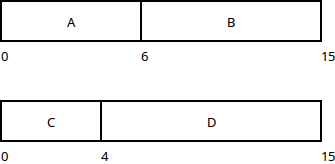
\includegraphics[scale=0.6]{resources/scheduling-normal.png}}\\
    \vspace{18pt}\hspace{24pt}
    \subfloat[]{\label{subfigure:scheduling_comparison_b}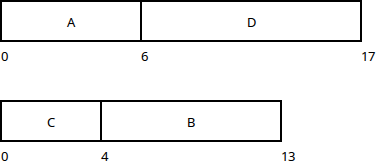
\includegraphics[scale=0.6]{resources/scheduling-realtime.png}}
    \caption[Ilustrasi perbedaan permasalahan \textit{scheduling} pada aplikasi \textit{real-time} dan \textit{non-real-time}]{Ilustrasi perbedaan permasalahan \textit{scheduling} pada aplikasi \textit{real-time} dan \textit{non-real-time}. (a) \textit{Scheduling} aplikasi \textit{non-real-time} (b) \textit{Scheduling} aplikasi \textit{real-time}}
    \label{figure:scheduling_comparison}
\end{figure}

Algoritma untuk \textit{scheduling} dapat diklasifikasikan dalam banyak dimensi.  Beberapa
algoritma \textit{scheduling} dibuat untuk \textit{periodic task} sedangkan algoritma lain
dibuat untuk \textit{aperiodic task}.  Demikian juga beberapa algoritma dibuat untuk
\textit{preemptible task} sedangkan algoritma lain dibuat untuk \textit{nonpreemptible task}.
Algoritma \textit{scheduling} dipengaruhi oleh faktor-faktor seperti tingkat kekritisan,
keterkaitan, \textit{resource}, dan \textit{deadline} aplikasi.

Algoritma \textit{scheduling} juga berbeda tergantung komputer tempat sistem akan dijalankan.
Beberapa faktor komputer yang memengaruhi algoritma \textit{scheduling} adalah arsitektur
\textit{processor} (\textit{uniprocessor} atau \textit{multiprocessor}), metode komunikasi
\textit{shared memory} atau \textit{message-passing}, dan jaringan.

\subsection{Arsitektur Sistem}

Standar ARINC 653 menspesifikasikan arsitektur sistem menggunakan arsitektur IMA.  Setiap
\textit{core module} dapat memiliki satu atau lebih \textit{processor}. Arsitektur dari
\textit{core module} memengaruhi implementasi sistem operasi, namun tidak memengaruhi
\textit{interface} APEX yang digunakan oleh \textit{aplikasi} pada masing-masing partisi.
Aplikasi harus mudah dipindahkan antar \textit{core module} dan antar \textit{processor} dari
sebuah \textit{core module} tanpa perlu adanya modifikasi \textit{interface} dengan sistem
operasi.  \autoref{figure:arinc653_module_architecture} menunjukkan contoh arsitektur sistem
ARINC 653 serta komunikasi antar komponen pada sistem.

\begin{figure}[htbp]
    \centering
    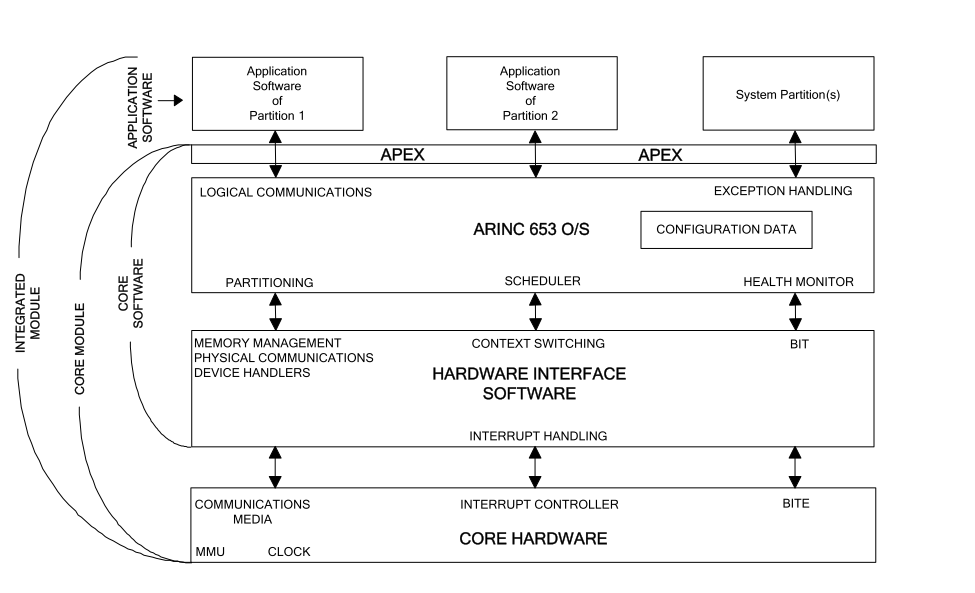
\includegraphics[scale=0.4]{resources/arinc653-architecture.png}
    \caption[Contoh arsitektur \textit{module}]{Contoh arsitektur \textit{module} \citep{AirlinesElectronicEngineeringCommittee2012}}
    \label{figure:arinc653_module_architecture}
\end{figure}

\subsection{Fungsionalitas Sistem}

Pada tingkat \textit{core module}, sistem operasi memanajemeni partisi dan komunikasi antar
partisi, yang mana mungkin dilakukan di dalam maupun antar \textit{module}.  Pada tingkat
partisi, sistem operasi memanajemeni proses aplikasi dalam sebuah partisi dan komunikasi antar
proses dalam partisi tersebut.  Sistem operasi menyediakan fasilitas pada kedua level tersebut,
namun memiliki perbedaan pada fungsi dan konten tergantung pada lingkup operasinya.  Maka,
definisi dari fasilitas yang diberikan sistem operasi membedakan pada tingkat apa fasilitas
tersebut beroperasi.

Pada setiap saat, sebuah \textit{module} berada dalam keadaan inisialisasi, operasional, atau
diam.  Pada saat dinyalakan, \textit{module} memulai eksekusinya dalam keadaan inisialisasi.
Setelah inisialisasi berhasil, \textit{module} masuk ke dalam keadaan operasional.  Selama
\textit{module} dalam keadaan operasional, sistem operasi memanajemeni partisi, proses aplikasi,
dan komunikasi.  \textit{Module} akan terus berada pada keadaan operasional sampai dimatikan
atau fungsi \textit{health monitoring} pada \textit{module} memerintahkan \textit{module} untuk
masuk ke dalam keadaan inisialisasi kembali atau keadaan diam.

Berikut adalah fungsionalitas sistem yang dispesifikasikan oleh standar ARINC 653.

\begin{enumerate}

    \item Manajemen Partisi.

    \item Manajemen Proses.

    \item Manajemen Waktu.

    \item Manajemen Memori.

    \item Komunikasi Antar Partisi.

    \item Komunikasi Dalam Partisi.

\end{enumerate}

Penelitian ini hanya akan membahas manajemen partisi dan manajemen waktu yang dilakukan oleh
ARINC 653.

\subsubsection[Manajemen Partisi]{Manajemen Partisi}

Inti dari standar ARINC 653 adalah konsep partisi, yaitu aplikasi yang beroperasi dalam sebuah
\textit{module} dipartisi terhadap ruang (partisi memori) dan waktu.  Sebuah partisi dapat
dikatakan sebagai satu unit aplikasi yang didesain untuk memenuhi batasan-batasan partisi.

Spistem operasi pada dasarnya sudah memiliki cara untuk melakukan partisi \textit{resource} yang
dimilikinya.  Sistem dengan partisi yang kuat memungkinkan partisi dengan tingkat kekritisan
yang berbeda berjalan pada satu \textit{module} yang sama tanpa memengaruhi partisi lain secara
\textit{ruang} dan waktu.  Bagian dari sistem operasi yang bekerja pada tingkat \textit{core
module} bertanggung jawab untuk melakukan partisi dan memanajemeni partisi dalam \textit{module}
tersebut.

Partisi ditentukan urutannya dengan melakukan \textit{scheduling} secara melingkar dan tetap.
Untuk dapat melakukan \textit{scheduling} secara melingkar, sistem operasi menyimpan
\textit{major time frame} untuk durasi tertentu yang kemudian akan diulang secara terus menerus
selama \textit{module} berjalan.  Partisi akan terdaftar pada \textit{major time frame} sebagai
\textit{partition window} yang memiliki nilai \textit{offset} sesuai dengan urutan yang telah
ditentukan.  Partisi dengan dijalankan terlebih dahulu akan mendaftarkan \textit{partition
window} dengan nilai \textit{offset} yang lebih kecil.  Urutan yang didapatkan oleh suatu
partisi ditentukan oleh pengaturan urutan yang dibuat pada saat integrasi.  Metode ini menjamin
bahwa \textit{scheduling} yang dilakukan akan bersifat deterministik sehingga dapat diprediksi.

Sebuah \textit{module} dapat memiliki beberapa partisi yang memiliki periode pengerjaan yang
berbeda-beda.  \textit{Major time frame} didefinisikan sebagai kelipatan dari kelipatan
persekutuan terkecil dari seluruh periode pengerjaan partisi pada \textit{module} tersebut.
Setiap \textit{major time frame} mempunyai partisi yang sama.  Periode pengerjaan masing-masing
partisi harus terpenuhi dengan mengatur frekuensi dan ukuran \textit{partition window} dalam
\textit{major time frame}.

\subsubsection{Manajemen Waktu}

Manajemen waktu adalah proses penting yang menjadi karakteristik sebuah sistem operasi yang
digunakan untuk sistem \textit{real-time}.  Waktu harus unik dan tidak bergantung pada eksekusi
partisi apa pun dalam \textit{module}.  Seluruh nilai waktu yang digunakan harus terkait dengan
waktu unik tersebut.  Sistem operasi menyediakan \textit{time-slicing} untuk
\textit{scheduling}, \textit{deadline}, \textit{periodicity} dari sebuah partisi.

Sebuah \textit{time capacity} terasosiasi dengan setiap proses.  \textit{Time capacity}
merepresentasikan waktu maksimal hasil perhitungan proses tersebut dapat digunakan untuk
memenuhi syarat proses tersebut telah berhasil dikerjakan.  Selama proses tersebut selesai
dikerjakan tanpa melebihi \textit{time capacity}-nya, \textit{deadline} proses tersebut
terpenuhi. Jika tidak, maka \textit{deadline} proses tersebut tidak terpenuhi dan sistem akan
menghasilkan \textit{error}.  \textit{Error} hasil \textit{deadline} yang tidak terpenuhi
menjadi acuan bahwa sistem tidak berhasil menjamin 100\% \textit{realtime}.

\section{\textit{Fault-Tolerant Partition Scheduling}}

Studi untuk membuat sistem \textit{real-time} menjadi \textit{fault-tolerant} telah banyak
dilakukan \citep{Campbell1986} \citep{Bertossi2006}. \citet{Campbell1986} menunjukkan penambahan
\textit{deadline} pada setiap \textit{task} akan menghasilkan sistem yang
\textit{fault-tolerant}.  Meski demikian, penambahan \textit{deadline} hanya menjamin waktu
\textit{response} sistem terhadap permintaan aplikasi dan hanya berfungsi sebagai indikator pada
saat melakukan verifikasi sistem.  \textit{Fault} yang dialami aplikasi tidak hanya berupa waktu
\textit{response} saja, sehingga metode tersebut hanya membuat sistem menjadi
\textit{fault-tolerant} secara parsial.  Untuk dapat mengatasi \textit{fault} yang tidak terduga
pada saat verifikasi maupun \textit{fault} pada proses verifikasi itu sendiri, salah satu solusi
yang diusulkan adalah dengan menggunakan skema \textit{primary-backup}.

Sebuah studi menunjukkan bahwa peningkatan keandalan \textit{hierarchical scheduler} seperti
\textit{scheduler} ARINC 653 dapat dilakukan dengan menggunakan skema \textit{primary-backup}
\citep{Hyun2012}. \textit{Primary-backup partition scheduling} merupakan proses
\textit{scheduling} yang terinspirasi oleh metode replikasi data. Pendekatan paling sederhana
untuk melakukan \textit{primary-backup partition scheduling} adalah dengan memberikan salinan untuk setiap
\textit{task}, dan memberikan salinan tersebut pada \textit{processor} yang berbeda dengan
\textit{task} aslinya.  Namun, pendekatan tersebut tidak efisien karena memerlukan banyak
\textit{processor} tambahan \citep{Oh1994}.  \citet{Bertossi2006} menunjukkan bagaimana cara
mengimplementasikan \textit{primary-backup partition scheduling} yang lebih efisien pada sistem
\textit{real-time} yang menggunakan algoritma \textit{scheduling} \textit{Rate-
Monotonic-First-Fit} (RMFF).  Implementasi tersebut memberikan \textit{task} \textit{salinan}
pada \textit{scheduler} jika dan hanya jika \textit{task} utama mengalami kegagalan.
\citet{Jin2013} berhasil membuktikan bahwa penggunaan \textit{primary-backup partition scheduling} dapat
dilakukan pada sistem \textit{uniprocessor} yang terpartisi dengan melakukan perluasan model
\textit{resource}.

\section{Virtualisasi}

Dalam ranah komputasi, virtualisasi adalah tindakan untuk membuat versi virtual dari suatu hal.
Virtualisasi pertama kali digunakan sekitar tahun 1960 sebagai metode untuk membagi
\textit{resources} sebuah komputer secara logika kepada beberapa aplikasi yang akan
menggunakannya.  Sejak saat itu, arti dari istilah virtualisasi mengalami perluasan makna.

Virtualisasi dapat dilakukan pada berbagai macam hal terkait dengan komputer.  Sebagai contoh,
sistem operasi modern sudah menggunakan konsep virtualisasi sederhana.  Sebuah sistem operasi
dapat mengatasi banyak aplikasi yang berjalan pada saat yang bersamaan yang mana masing-masing
membutuhkan \textit{resources} agar dapat berjalan sebagaimana seharusnya.  Dalam kasus ini,
sistem operasi memberikan ilusi kepada masing-masing proses bahwa proses tersebut memiliki
seluruh \textit{resources} yang terdapat pada komputer tersebut.  Namun, yang terjadi adalah
sistem operasi membagi \textit{resources} komputer dengan metode sedemikian rupa sehingga
pemakaian \textit{resources} tetap konsisten dengan ilusi yang diberikan oleh sistem operasi
kepada masing-masing proses.

Sebagai contoh, virtualisasi CPU dilakukan dengan melakukan \textit{preemption} pada proses yang
sedang menggunakan CPU sehingga memberikan kesempatan bagi proses lain untuk menggunakan CPU.
Sistem operasi melakukan melakukan \textit{context switch} pada proses yang terkena
\textit{preemption} sehingga pada proses saat tersebut mendapatkan CPU pada giliran selanjutnya,
proses tersebut dapat melanjutkan apa yang dikerjakan sebelumnya.  Sementara itu, virtualisasi
memori yang dilakukan dengan melakukan pemetaan alamat memori virtual yang mampu memiliki
kapasitas 2\textsuperscript{32} (2\textsuperscript{64} pada sistem 64-bit) ke alamat memori
fisik yang memiliki kapasitas sesuai dengan perangkat keras komputer.  Kapasitas yang dapat
digunakan oleh sebuah proses pada alamat memori fisik serta cara pemetaannya dilakukan oleh
perangkat MMU pada komputer.  \textit{Devices} yang dimiliki oleh sebuah komputer juga
divirtualisasikan oleh sistem operasi.  Contoh \textit{device} yang divirtualisasikan oleh
sistem operasi adalah \textit{storage}.

Salah satu kegunaan metode virtualisasi pada ranah komputasi adalah untuk membuat
\textit{virtual machine}.  Sebuah \textit{virtual machine} adalah representasi mesin secara
logika yang memiliki \textit{resources} layaknya mesin biasa.  Umumnya, \textit{virtual machine}
digunakan untuk memberikan ilusi sebuah komputer sehingga dari sudut pandang perangkat lunak
yang berjalan di atasnya, perangkat lunak tersebut seakan berjalan satu buah komputer fisik
tanpa ada pembagian \textit{resources}.  Tentunya hal tersebut hanya berlaku untuk sistem
operasi atau perangkat lunak yang berjalan langsung di atas perangkat keras.  Sebuah komputer
dapat direpresentasikan menjadi beberapa \textit{virtual machine} sehingga memungkinkan beberapa
sistem operasi beroperasi secara bersamaan pada komputer tersebut.

\section{\textit{Hypervisor}}

Virtualisasi dilakukan menggunakan perangkat lunak virtualisasi yang disebut sebagai
\textit{hypervisor}.  \textit{Hypervisor} adalah sebuah perangkat lunak yang bertugas untuk
membuat dan menjalankan beberapa \textit{virtual machine}.  \textit{Hypervisor} berfungsi untuk
memanajemeni \textit{resources} fisik yang tersedia untuk digunakan oleh \textit{virtual
machine} yang berjalan di bawah \textit{hypervisor} tersebut.  Dengan demikian,
\textit{hypervisor} memiliki peran sama seperti sistem operasi, hanya saja ketimbang
memanajemeni \textit{resources} fisik untuk digunakan oleh proses perangkat lunak,
\textit{hypervisor} memanajemeni \textit{resources} untuk sebuah proses yang juga mengatur
\textit{resources} yang diberikan pada proses tersebut untuk proses perangkat lunak yang
berjalan di bawahnya.  Istilah \textit{hypervisor} didapatkan karena \textit{hypervisor}
membawahkan \textit{supervisor}, pada kasus ini \textit{supervisor}-nya merupakan sistem
operasi.

\section{Xen}

Xen merupakan sebuah perangkat lunak untuk melakukan virtualisasi yang bekerja diantara sistem
operasi dan perangkat keras.  Xen menyediakan lingkungan virtual yaitu sebuah \textit{kernel}
dapat beroperasi.  Terdapat tiga komponen utama pada sistem yang menggunakan Xen, yaitu
\textit{hypervisor}, \textit{kernel}, dan aplikasi yang bekerja pada \textit{userspace}.

\begin{figure}[h]
    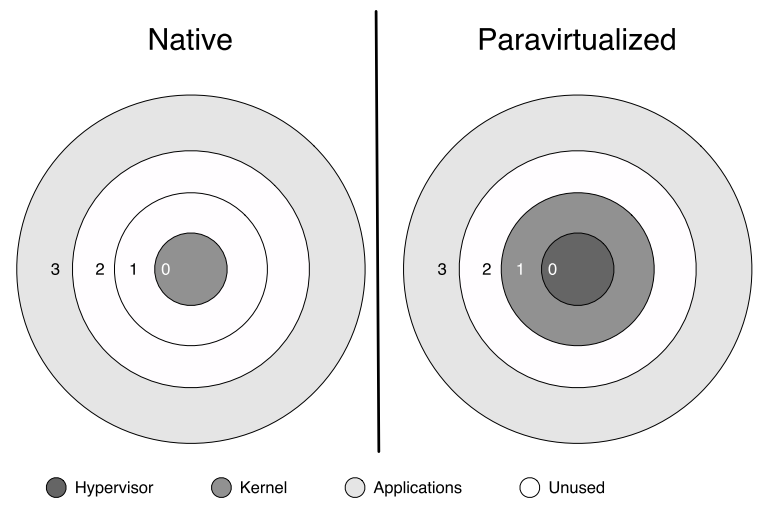
\includegraphics[scale=0.5]{./resources/xen-ring.png}
    \caption[Perbedaan penggunaan \textit{ring} \textit{native} dan
    \textit{paravirtualized}]{Perbedaan penggunaan \textit{ring} \textit{native} (kiri) dan
    \textit{paravirtualized} (kanan) \citep{Chisnall2014}}
    \label{figure:xen_ring}
\end{figure}

Pada Xen, \textit{kernel} sebuah sistem operasi tidak lagi beroperasi pada \textit{ring} 0.
\textit{Ring} 0 digunakan oleh \textit{hypervisor} yang akan mengatur \textit{resources} yang
akan diberikan pada \textit{virtual machine} di bawahnya.  \textit{Kernel} sistem operasi
dijalankan bergantung pada arsitektur \textit{processor}-nya.  Sebagai contoh, pada sistem IA32,
\textit{kernel} sistem operasi berjalan pada \textit{ring} 1 seperti pada
\autoref{figure:xen_ring}.  Hal tersebut mengakibatkan \textit{kernel} yang berjalan di atas Xen
tetap dapat mengakses memori yang teralokasi untuk aplikasi yang berjalan di atas kernel
tersebut, namun tetap tidak dapat diakses oleh aplikasi maupun \textit{kernel} lain.
\textit{Hypervisor}, yang berjalan pada \textit{ring} 0, terproteksi dari \textit{kernel} yang
berjalan pada \textit{ring} 1 dan aplikasi yang berjalan pada \textit{ring} 3.  Karena
\textit{kernel} berjalan pada \textit{ring} 1, \textit{kernel} tidak dapat menjalankan
\textit{privileged instructions} seperti biasanya.  \textit{Hypervisor} pada Xen menyediakan
\textit{hypercall} sebagai pengganti \textit{privileged instructions}.

\begin{figure}[h]
    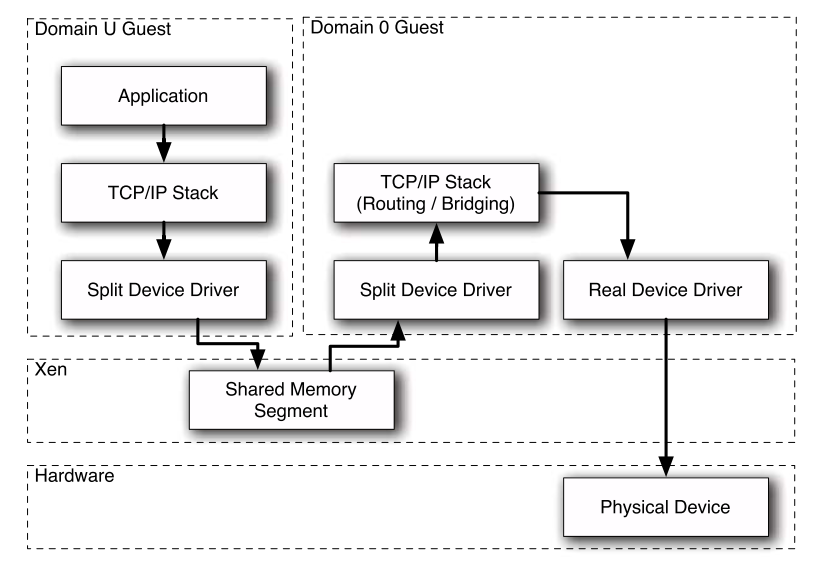
\includegraphics[scale=0.5]{./resources/xen-split-driver.png}
    \caption[Jalur sebuah paket jaringan yang dikirim dari domU]{Jalur sebuah paket jaringan yang dikirim dari domU \citep{Chisnall2014}}
    \label{figure:xen_split_driver}
\end{figure}

Fungsi dari sebuah \textit{hypervisor} adalah untuk menjalankan \textit{virtual machine}.  Pada
Xen, \textit{hypervisor} menjalankan \textit{virtual machine} yang disebut sebagai
\textit{domain}.  Terdapat dua jenis \textit{domain} pada Xen, yaitu dom0 dan domU.  Dom0
merupakan \textit{domain} yang memiliki \textit{privileged instructions} untuk memanajemeni
\textit{devices} yang dijalankan oleh Xen pada saat sistem pertama kali beroperasi.  Kewajiban
dom0 dalam menangani \textit{devices} adalah dom0 harus dapat menyediakan \textit{devices} untuk
semua domU.  Karena perangkat keras tidak dapat diakses oleh beberapa sistem operasi sekaligus,
maka akses \textit{devices} oleh domU harus melalui dom0.  \autoref{figure:xen_split_driver}
mengilustrasikan bagaimana paket jaringan yang dikirim oleh domU melalui dom0.  Perbedaan utama
pada pengiriman paket jaringan adalah pada \textit{layer} \textit{TCP/IP}, \textit{layer}
tersebut tidak meneruskan langsung ke \textit{network device} tetapi menulis paket pada
\textit{shared memory}.  Kemudian dom0 akan membaca paket yang terdapat pada \textit{shared
memory} untuk dilanjutkan ke \textit{network device} yang sebenarnya.  Penggunaan \textit{shared
memory} seperti ilustrasi tersebut banyak digunakan pada berbagai komponen yang membentuk Xen.

Salah satu kelebihan Xen sebagai \textit{hypervisor} adalah Xen memudahkan pengembang untuk
menuliskan komponen sesuai dengan kebutuhan.  Xen menjelaskan secara rinci bagaimana proses
penulisan komponen dan memberikan \textit{interface} yang relatif mudah.  Xen juga merupakan
\textit{hypervisor} \textit{open-source}, sehingga eksplorasi keseluruhan sistem lebih mudah
dilakukan.  Fokus utama pada buku ini adalah, Xen menyediakan \textit{interface} untuk membuat
\textit{scheduler} baru.  \textit{Scheduler} dalam kasus ini tidak bekerja pada proses,
tetapi bekerja pada \textit{domain}.

\section{ARLX}

ARLX merupakan prototipe sistem ARINC 653 yang dibangun di atas Xen.  Prototipe dibangun dengan
membuat \textit{scheduler} seperti pada spesifikasi standar ARINC 653 pada Xen.  Selain itu,
prototipe tersebut memberikan beberapa modul \textit{kernel} untuk menangani \textit{device}
yang terpartisi sesuai dengan spesifikasi ARINC 653. Dalam melakukan partisi memori, prototipe
tersebut memanfaatkan mekanisme partisi memori menggunakan MMU yang sudah merupakan mekanisme
bawaan pada Xen.

\begin{figure}[!ht]
    \centering
    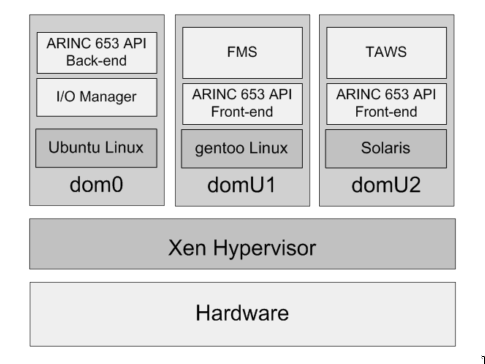
\includegraphics[scale=0.6]{resources/xen-arinc653-partitions.png}
    \caption{\textit{Hypervisor} ARLX}
    \label{figure:xen_arinc653_partitions}
\end{figure}

Setiap partisi akan direpresentasikan dengan menggunakan \textit{domain} pada Xen.  Dom0 pada
Xen akan digunakan sebagai partisi tempat APEX dan \textit{device driver} berada, sedangkan
partisi untuk aplikasi avionik akan direpresentasikan menggunakan domU seperti pada
\autoref{figure:xen_arinc653_partitions}.

\textit{Partition scheduling} dilakukan seperti yang telah dispesifikasikan pada standar ARINC
653. Layanan sebuah partisi akan didaftarkan dengan menggunakan \textit{hypercall}. Partisi
akan dipilih sesuai dengan urutan yang diberikan pada saat melakukan \textit{hypercall}.
Ilustrasi penjadwalan partisi yang dilakukan oleh \textit{partition scheduler} milik ARLX dapat
dilihat pada \autoref{figure:xen_arinc653_partitions_schedule}. Algoritma ini bekerja untuk
sebuah \textit{major time frame} dan akan dilakukan secara terus menerus untuk setiap
\textit{major time frame}.

\begin{figure}[!hb]
    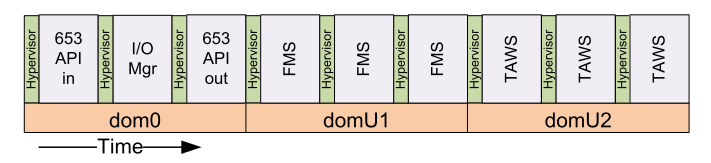
\includegraphics[scale=0.6]{resources/xen-arinc653-partition-schedule.png}
    \caption{\textit{Schedule} partisi pada ARLX}
    \label{figure:xen_arinc653_partitions_schedule}
\end{figure}

% vim: tw=96
